\documentclass{article}

\usepackage{tikz}

\usetikzlibrary{fpu}
\usetikzlibrary{math}


\begin{document}

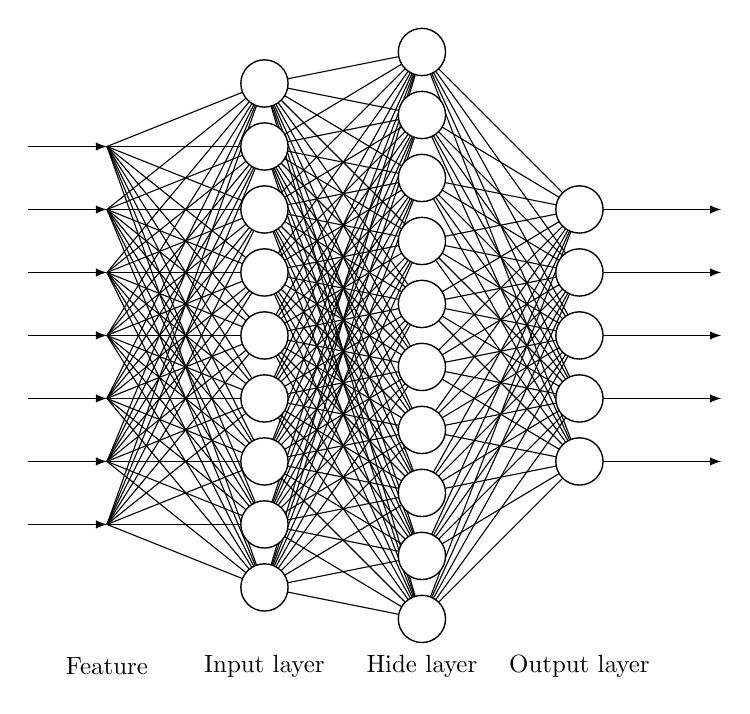
\begin{tikzpicture} 
    \tikzmath{ 
        function paint_nodes(\radius,\gapy,\posx,\num){ 
            \gapy = \gapy+\radius*2;  
            \starty = \gapy*(\num-1)/2; 
            for \i in {0,...,\num-1}{
                \drawy = \starty - \i*\gapy; 
                {
                    \filldraw[line width = 0.5pt,fill = white] (\posx,\drawy) circle (\radius);
                };
            };   
        };
        function paint_lines(\radius,\gapy,\posx,\num,\nextposx,\nextnum){ 
            \gapy = \gapy+\radius*2;  
            \starty = \gapy*(\num-1)/2;
            \startyy = \gapy*(\nextnum-1)/2; 
            for \i in {0,...,\num-1}{
                \drawy = \starty - \i*\gapy; 
                for \j in {0,...,\nextnum-1}{  
                    \drawyy = \startyy - \j*\gapy;   
                    {
                        \draw (\posx,\drawy) -- (\nextposx,\drawyy);
                    };
                }; 
            };
        };
        function paint_x_lines(\radius,\gapy,\posx,\num,\ifright,\len){
            \gapy = \gapy+\radius*2;  
            \starty = \gapy*(\num-1)/2; 
            for \i in {0,...,\num-1}{
                \drawy = \starty - \i*\gapy; 
                if \ifright == 1 then{
                    {
                        \draw[-latex] (\posx,\drawy) -- (\posx+\len,\drawy);
                    }; 
                }else{ 
                    {
                        \draw[-latex] (\posx,\drawy)--(\posx-\len,\drawy);
                    }; 
                }; 
            }; 
        };
        function paint_net(\x0,\x1,\x2,\x3){  
            \gapx = 2;
            \radius = 0.3;
            \gapy = 0.2; 
            paint_lines(\radius,\gapy,0*\gapx,\x0,1*\gapx,\x1);
            paint_lines(\radius,\gapy,1*\gapx,\x1,2*\gapx,\x2);
            paint_lines(\radius,\gapy,2*\gapx,\x2,3*\gapx,\x3); 
            paint_x_lines(\radius,\gapy,3*\gapx,\x3,1,1.8);
            paint_x_lines(\radius,\gapy,0*\gapx-1,\x0,1,1);
            paint_nodes(\radius,\gapy,1*\gapx,\x1); 
            paint_nodes(\radius,\gapy,2*\gapx,\x2);
            paint_nodes(\radius,\gapy,3*\gapx,\x3);  
        };  
        paint_net(7,9,10,5); 
    } 
    \node[scale = 0.9] at (0,-4.2) {Feature};
    \node[scale = 0.9] at (2,-4.2) {Input layer};
    \node[scale = 0.9] at (4,-4.2) {Hide layer};
    \node[scale = 0.9] at (6,-4.2) {Output layer}; 

\end{tikzpicture}

\end{document}